% This LaTeX was auto-generated from MATLAB code.
% To make changes, update the MATLAB code and export to LaTeX again.

\documentclass{article}

\usepackage[utf8]{inputenc}
\usepackage[T1]{fontenc}
\usepackage{lmodern}
\usepackage{graphicx}
\usepackage{color}
\usepackage{hyperref}
\usepackage{amsmath}
\usepackage{amsfonts}
\usepackage{epstopdf}
\usepackage[table]{xcolor}
\usepackage{matlab}

\sloppy
\epstopdfsetup{outdir=./}
\graphicspath{ {./Lab05_images/} }

\begin{document}

\matlabtitle{LAB 5: ANGULAR VELOCITY CONTROL FOR DC MOTOR}

\begin{matlabcode}
%---------------------------------------
% Fill in your student Name and ID.
Students.Name = 'Seyed Yazdan Zinati';
Students.ID = '260928077';
%---------------------------------------
\end{matlabcode}


\matlabheading{\textbf{0. Objectives}}

\begin{par}
\begin{flushleft}
In this lab, we will design an angular velocity state-feedback controller to track a desired reference signal. First, we will run an open-loop experiment to get an understanding about the normal system dynamics. Second, we will design a theoretical state-feedback controller based on a DC Motor model. Finally, we will tune the gains of the controller on the Virtual Motor to account for modeling uncertainties and sensor noise.
\end{flushleft}
\end{par}

\begin{par}
\begin{flushleft}
To initiate a connection with the virtual motor, run the following:
\end{flushleft}
\end{par}

\begin{matlabcode}
Motor = VirtualMotor();
\end{matlabcode}


\matlabheading{\textbf{1. A State-Space Representation of DC Motor}}

\begin{par}
\begin{flushleft}
A DC motor is a device that converts armature current into mechanical torque. A schematic of a DC motor is shown in the following
\end{flushleft}
\end{par}

\begin{par}
\begin{flushleft}
\textless{}\textless{}fig\_dcmotorshematic.png\textgreater{}\textgreater{}
\end{flushleft}
\end{par}

\begin{par}
\begin{flushleft}
We can model the DC motor using the armature current $i$ and the angular speed $\omega$. The dynamics of the DC motor are given by the following two coupled differential equations:
\end{flushleft}
\end{par}

\begin{par}
$$J{{\frac{d\omega }{dt}+b\omega =K_t i}}$$
\end{par}

\begin{par}
$$L{{\frac{di}{dt}+Ri=v-K_e \omega }}$$
\end{par}

\begin{par}
\begin{flushleft}
where the parameters are defined as follow
\end{flushleft}
\end{par}

\begin{matlabcode}
Param.Kt = 0.034; % Torque proportionality constant (Kg m2 /s2/A) (N.m/A)
Param.Ke = 0.034; % Back electromotive proportionality constant (V/rad/s)
Param.L = 0.018; % Electric inductance (H)
Param.R = 8.4; % Terminal resistance (Ohm)
Param.J = 2e-05; % Rotor moment of inertia (kg.m2)
Param.b = 1e-06; % Rotor viscous friction constant (Kg.m2/s) (N.m.s)
\end{matlabcode}


\begin{par}
\begin{flushleft}
From these differential equations we can represent the DC Motor model by the following state-space representation
\end{flushleft}
\end{par}

\begin{par}
$${{\frac{d}{dt}x(t)=\left(\begin{array}{cc}
-{{\frac{b}{J}}} & {{\frac{K_t }{J}}}\\
-{{\frac{K_e }{L}}} & -{{\frac{R}{L}}}
\end{array}\right)x(t)+\left(\begin{array}{c}
0\\
{{\frac{1}{L}}}
\end{array}\right)v(t)}}$$
\end{par}

\begin{par}
\begin{flushleft}
where $v(t)$ is the voltage and the state vector contains the angular velocity $\omega (t)$ and the current $i(t)$
\end{flushleft}
\end{par}

\begin{par}
$$x(t)=\left(\begin{array}{c}
\omega (t)\\
i(t)
\end{array}\right)$$
\end{par}

\begin{par}
\begin{flushleft}
Note that if we think of the angular velocity $\omega (t)$ as the output of this system, then $C=\left(\begin{array}{cc}
1 & 0
\end{array}\right)$ and
\end{flushleft}
\end{par}

\begin{par}
$$\omega (t)=Cx(t)$$
\end{par}

\begin{par}
\begin{flushleft}
In this case, the transfer function from the voltage $v(t)$ to the angular velocity $\omega (t)$ is given by
\end{flushleft}
\end{par}

\begin{par}
$$G_o (s)=C(sI-A)^{-1} B$$
\end{par}

\begin{par}
\begin{flushleft}
The state-space representation of the DC Motor can be written as
\end{flushleft}
\end{par}

\begin{matlabcode}
A = [ ...
    -Param.b / Param.J, Param.Kt / Param.J; ...
    -Param.Ke / Param.L, -Param.R / Param.L];
B = [ ...
    0; ...
    1 / Param.L];
C = [1, 0];
D = 0;
Go = ss(A, B, C, D);
tf(Go)
\end{matlabcode}
\begin{matlaboutput}
ans =
 
        9.444e04
  --------------------
  s^2 + 466.7 s + 3234
 
Continuous-time transfer function.
\end{matlaboutput}


\matlabheading{\textbf{2. Desired specifications}}

\begin{par}
\begin{flushleft}
The objective of this lab is to track a reference signal $\omega_{ref}$ while satisfying the following requirements:
\end{flushleft}
\end{par}

\begin{itemize}
\setlength{\itemsep}{-1ex}
   \item{\begin{flushleft} Overshoot less than 20\%. \end{flushleft}}
   \item{\begin{flushleft} 5\%-settling time less than 0.25 seconds. \end{flushleft}}
   \item{\begin{flushleft} Steady state gain of 1 $\pm$ 5\%. \end{flushleft}}
\end{itemize}

\begin{par}
\begin{flushleft}
The Reference angular velocity is defined by the following:
\end{flushleft}
\end{par}

\begin{par}
$$\omega_{ref} (t)=\left\lbrace \begin{array}{cc}
25, & 0\le t<5\\
75, & t\ge 5
\end{array}\right.$$
\end{par}

\begin{par}
\begin{flushleft}
In \texttt{\textbf{MATLAB}} we define $\omega_{ref}$ by:
\end{flushleft}
\end{par}

\begin{matlabcode}
T = 10; % Simulation duration
dt = 0.01; % Simulation step time
t = (0:dt:T)'; % Time array
TStart = 5; % Step start
wRef = zeros(size(t));
wRef(t < TStart) = 25; % rad/s
wRef(t >= TStart) = 75; % rad/s

figure;
clf;
plot(t, wRef, 'LineWidth', 2.0)
legend('Reference angular velocity (rad/s)');
xlim([0, T])
ylim([0, 100])
title(sprintf('Student ID %s - Reference angular velocity', Students.ID));
grid on
\end{matlabcode}
\begin{center}
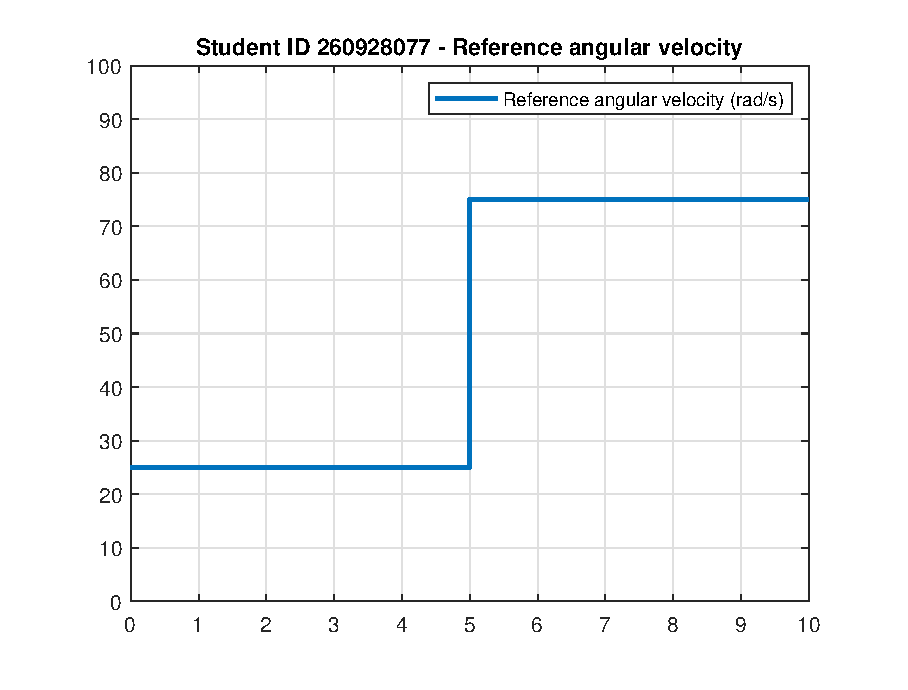
\includegraphics[width=\maxwidth{56.196688409433015em}]{figure_0.eps}
\end{center}


\matlabheading{\textbf{3. Open-loop Experiment}}

\begin{par}
\begin{flushleft}
The state-space open-loop system is presented below.
\end{flushleft}
\end{par}

\begin{par}
\begin{flushleft}
\textless{}\textless{}fig\_lab04\_openloopdiagram.png\textgreater{}\textgreater{}
\end{flushleft}
\end{par}

\begin{par}
\begin{flushleft}
The gain $N_o$ is used to compensate for the open-loop DC gain, such as the total gain from $\omega_{ref}$ to $\omega$ is one.
\end{flushleft}
\end{par}

\matlabheading{\textit{Question 1 (2 marks)}}

\begin{par}
\begin{flushleft}
Complete the following code to run the DC Motor in open-loop in such a way that the angular velocity $\omega (t)$ follows the desired angular velocity signal $\omega_{ref}$
\end{flushleft}
\end{par}

\begin{matlabcode}
% Determine a pre compensator N_o
dcGainOL = dcgain(Go)
\end{matlabcode}
\begin{matlaboutput}
dcGainOL = 29.1996
\end{matlaboutput}
\begin{matlabcode}
N_o = 1/dcGainOL
\end{matlabcode}
\begin{matlaboutput}
N_o = 0.0342
\end{matlaboutput}
\begin{matlabcode}

% Run the experiment
Motor.reset();


% value of the voltage v
v = N_o*wRef;

Motor.input(v);
Motor.off();

Motor.save(Students, 'Lab05.Q1');
\end{matlabcode}


\begin{matlabcode}
% Get results of driving Virtual DC Motor
v = Motor.voltage(Motor.time <= T);
i = Motor.current(Motor.time <= T);
w = Motor.velocity(Motor.time <= T);

% Plot results
figure;
clf;


% Superpose the angular velocity w and the reference wRef
plot(t, w)
hold on
plot(t, wRef)
hold off

legend('Angular velocity (rad/s)', ...
    'Reference angular velocity (rad/s)', ...
    'location', 'best');
xlim([TStart - 1, T])
ylim([0, 100])
title(sprintf('Student ID %s - Open-loop tracking experiment', Students.ID));
grid on
\end{matlabcode}
\begin{center}
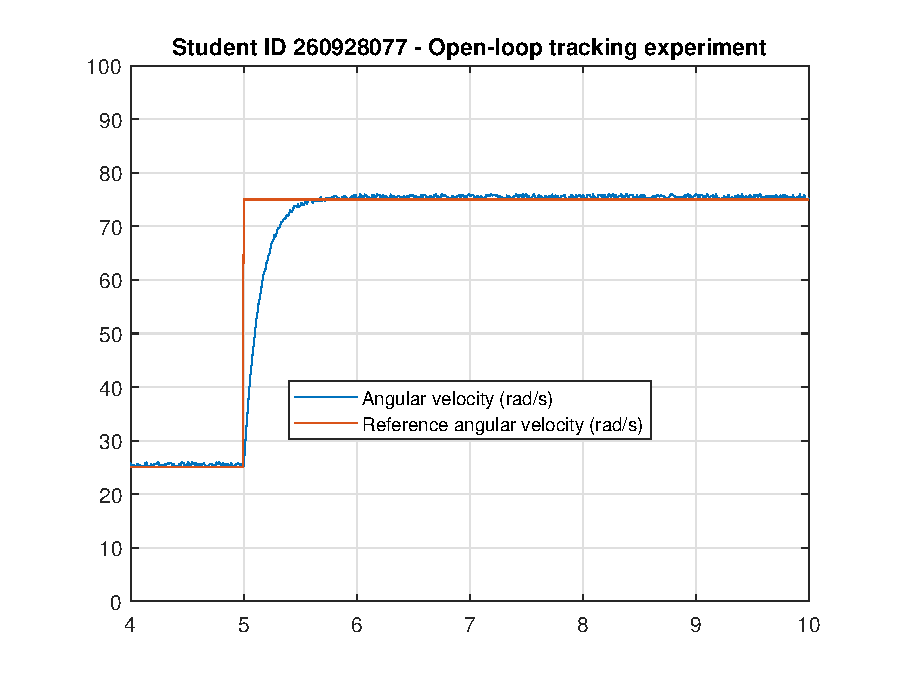
\includegraphics[width=\maxwidth{56.196688409433015em}]{figure_1.eps}
\end{center}


\matlabheading{\textit{Question 2 (0.5 marks)}}

\begin{par}
\begin{flushleft}
Based on the plot above, determine if all the requirements are satisfied. Justify your answer.
\end{flushleft}
\end{par}

\begin{par}
\begin{flushleft}
Answer here
\end{flushleft}
\end{par}

\begin{matlabcode}
stepinfo(w,"SettlingTimeThreshold", 0.05)
\end{matlabcode}
\begin{matlaboutput}
ans = 
        RiseTime: 521.1658
    SettlingTime: 537.5700
     SettlingMin: 68.0195
     SettlingMax: 75.9975
       Overshoot: 1.0236
      Undershoot: 0
            Peak: 75.9975
        PeakTime: 824

\end{matlaboutput}
\begin{matlabcode}

% The objective was to track a signal ωrefwhile satisfying the following requirements:
% • Overshoot less than 20%.
% • 5%-settling time less than 0.25 seconds.
% • Steady state gain of 1±5%.

% As we see from the plot, there is a slight overshoot that can bee seen
% from w. Using stepinfo() we see that the overshoot is 0.2439% < 20%. So Overshoot
% requirements are met. 

% The settling time is: 
5.381019 - 5
\end{matlabcode}
\begin{matlaboutput}
ans = 0.3810
\end{matlaboutput}
\begin{matlabcode}
% which is larger than 0.25 seconds so the requirement for settling time is
% not met (0.381019s > 0.25s)

% We can find the steady state gain as follows : 
finalW = mean(w(t>=6));
finalWred = mean(wRef(t>=6));
SSgain = finalW/finalWred
\end{matlabcode}
\begin{matlaboutput}
SSgain = 1.0068
\end{matlaboutput}
\begin{matlabcode}
% We can see that the SS gain is equal to 1.00668 which lies in our error
% bound. So ss gain requirements are met. 

% OS and SSgain requirements are met while Settling time requirements are not.
% Not all requirements are satisfied. 

\end{matlabcode}

\matlabheading{\textbf{4. Closed-Loop Simulation Experiment}}

\begin{par}
\begin{flushleft}
The closed-loop system is presented in the following figure.
\end{flushleft}
\end{par}

\begin{par}
\begin{flushleft}
\textless{}\textless{}fig\_lab04\_clsoedloopdiagram1.png\textgreater{}\textgreater{}
\end{flushleft}
\end{par}

\begin{par}
\begin{flushleft}
The full-state feedback control law is defined as follow
\end{flushleft}
\end{par}

\begin{par}
$$v(t)=N_c \omega_{ref} -Kx(t)$$
\end{par}

\begin{par}
\begin{flushleft}
where gain $K$ is a 1 by 2 matrix and the gain $N_c$ is forward gain that will ensure achieving $\omega_{ref}$ at steady state.
\end{flushleft}
\end{par}

\begin{par}
\begin{flushleft}
Actually, this diagram is equivalent to an open-loop diagram but with a different state transition matrix $A_{cl} =A-BK$
\end{flushleft}
\end{par}

\begin{par}
\begin{flushleft}
\textless{}\textless{}fig\_lab04\_clsoedloopdiagram2.png\textgreater{}\textgreater{}
\end{flushleft}
\end{par}

\begin{par}
\begin{flushleft}
Doing a state feedback with gain $K$ is equivalent to changing the system dynamics from $A$ to $A-BK$. Recall that the eigenvalues of a state transition matrix $A$ are the poles of the system.
\end{flushleft}
\end{par}

\begin{par}
\begin{flushleft}
We want to choose $K$ to specify the new poles of the closed-loop system $A-BK$ in a way that satisfies the desired specifications
\end{flushleft}
\end{par}

\begin{itemize}
\setlength{\itemsep}{-1ex}
   \item{\begin{flushleft} Overshoot less than 20\%. \end{flushleft}}
   \item{\begin{flushleft} 5\%-settling time less than 0.25 seconds. \end{flushleft}}
\end{itemize}

\begin{par}
\begin{flushleft}
Then we will choose $N_c$ similarly to the open-loop section to satisfy the steady state requirements:
\end{flushleft}
\end{par}

\begin{itemize}
\setlength{\itemsep}{-1ex}
   \item{\begin{flushleft} Steady state gain of 1 $\pm$ 5\%. \end{flushleft}}
\end{itemize}

\matlabheading{\textit{Question 3 (2 marks)}}

\begin{par}
\begin{flushleft}
Calculate the desired poles that satisfies the specifications (Use formula sheet for transient response of 2nd order system in myCourses if needed). And find the gain $K$ that place the poles of $A-BK$ at the desired poles (Use \texttt{\textbf{place}}).
\end{flushleft}
\end{par}

\begin{matlabcode}
% find zeta based on the overshoot percentage
os = 20/100;
zeta = -(log(os))/sqrt(pi.^2 + (log(os)).^2)
\end{matlabcode}
\begin{matlaboutput}
zeta = 0.4559
\end{matlaboutput}
\begin{matlabcode}

% find wn based on the 5% settling time and zeta
ts = 0.25
\end{matlabcode}
\begin{matlaboutput}
ts = 0.2500
\end{matlaboutput}
\begin{matlabcode}
wn = 3/(zeta*ts)
\end{matlabcode}
\begin{matlaboutput}
wn = 26.3187
\end{matlaboutput}
\begin{matlabcode}

% find the roots of the TF
p = [1 2*wn*zeta wn^2];
r = roots(p);

% I hate that arrays start at 1. So counterintuitive 
p1d = r(1)
\end{matlabcode}
\begin{matlaboutput}
p1d = -12.0000 + 23.4238i
\end{matlaboutput}
\begin{matlabcode}
p2d = r(2)
\end{matlabcode}
\begin{matlaboutput}
p2d = -12.0000 - 23.4238i
\end{matlaboutput}
\begin{matlabcode}

K = place(A, B, [p1d, p2d]);
\end{matlabcode}


\matlabheading{\textit{Question 4 (1 mark)}}

\begin{itemize}
\setlength{\itemsep}{-1ex}
   \item{\begin{flushleft} The closed-loop transfer function is \end{flushleft}}
\end{itemize}

\begin{par}
$$G_c (s)=C(sI-(A-BK))^{-1} B$$
\end{par}

\begin{enumerate}
\setlength{\itemsep}{-1ex}
   \item{\begin{flushleft} What is the value of the DC gain of the closed-loop system. \end{flushleft}}
   \item{\begin{flushleft} What is the value $N_c$ needed to compensate for the DC gain of the closed-loop system. \end{flushleft}}
\end{enumerate}

\begin{matlabcode}
Gc = ss((A-B*K), B, C, D);
tf(Gc)
\end{matlabcode}
\begin{matlaboutput}
ans =
 
       9.444e04
  ------------------
  s^2 + 24 s + 692.7
 
Continuous-time transfer function.
\end{matlaboutput}
\begin{matlabcode}

dcGainCL = dcgain(Gc)
\end{matlabcode}
\begin{matlaboutput}
dcGainCL = 136.3478
\end{matlaboutput}


\begin{matlabcode}
Nc = 1/dcGainCL
\end{matlabcode}
\begin{matlaboutput}
Nc = 0.0073
\end{matlaboutput}


\matlabheading{\textit{Question 5 (1 mark)}}

\begin{par}
\begin{flushleft}
Complete the following to simulate angular velocity control with state feedback that tracks the desired $\omega_{ref}$.
\end{flushleft}
\end{par}

\begin{matlabcode}
% Define the closed-loop system using ss

% Gc = ss((A-B*K), B, C, D); (Already defined above)


% Simulate the output angular velocity using lsim

wSim = lsim(Gc, Nc*wRef, t);


% We also simulate the voltage for visualization
vSim = -lsim(ss(Gc.A, Gc.B, eye(2), Gc.D), Nc*wRef, t) * K' + Nc * wRef;

figure;
clf;

subplot(2, 1, 1)
% Superpose the simulated angular velocity wSim with the
% angular velocity reference

plot(t, wSim)
hold on
plot(t, wRef)
hold off

legend('Simulated angular velocity (rad/s)', ...
    'Reference angular velocity (rad/s)', ...
    'location', 'best');
xlim([TStart-1, T])
ylim([0, 100])
grid on
title(sprintf('Student ID %s - Closed-loop tracking Simulation', Students.ID));

subplot(2, 1, 2)
% Plot the simulated voltage input
plot(t, vSim)
legend('voltage (V)', 'location', 'best');
xlim([TStart-1, T])
grid on
\end{matlabcode}
\begin{center}
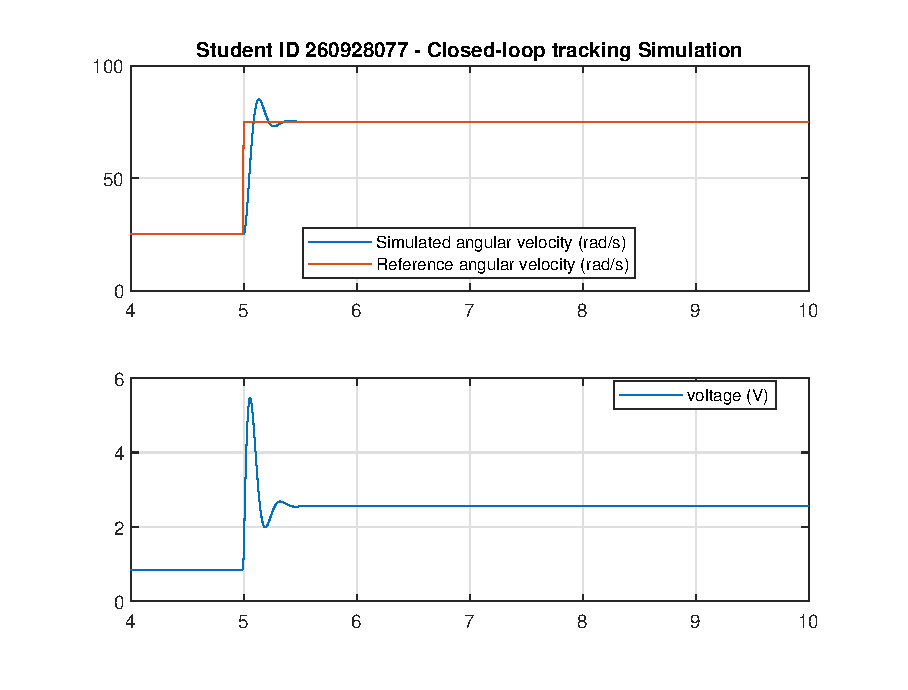
\includegraphics[width=\maxwidth{56.196688409433015em}]{figure_2.eps}
\end{center}


\matlabheading{\textit{3.2. Closed-loop Experiment}}

\begin{par}
\begin{flushleft}
In order to control the virtual DC Motor, we need to take into account the sampling time $\delta t$. For this, we generate a discrete control law that achieves the desired poles.
\end{flushleft}
\end{par}

\begin{matlabcode}
Go_d = c2d(Go, dt, 'zoh'); % get the equivalent discrete open-loop system
Kd = place(Go_d.A, Go_d.B, [exp(p1d*dt), exp(p2d*dt)]);
Nd = 1 / (Go_d.C * (eye(2) - Go_d.A + Go_d.B * Kd)^(-1) * Go_d.B);
\end{matlabcode}


\begin{par}
\begin{flushleft}
The gains $K_d$ and $N_d$ are the discrete equivalent of the gains $K$ and $N_c$. we will use these gains ($K_d$ and $N_d$) instead to control the virtual DC Motor.
\end{flushleft}
\end{par}

\begin{par}
\begin{flushleft}
Observe that now in closed-loop the value of the voltage (the control law) changes every time depending on the new value of $x(t)$, or in other words $\omega (t)$ and $i(t)$. To do this we will create a \texttt{\textbf{for}} loop that will loop over the time signal $t$. At every instant: \# we will wait for the Motor time to sync with our time signal, using the \texttt{\textbf{wait}} command. \# we will read new values of $\omega (t)$ and $i(t)$. \# we will generate the new voltage to send. \# we will send the voltage using \texttt{\textbf{input}} command.
\end{flushleft}
\end{par}

\matlabheading{\textit{Question 6 (2 marks)}}

\begin{par}
\begin{flushleft}
Complete the following to test the state feedback controller for tracking the desired $\omega_{ref}$. Observe that the control starts at time $t\ge T_{Start}$.
\end{flushleft}
\end{par}

\begin{matlabcode}
% Run the experiment
Motor.reset();
for n = 1:length(t)
    Motor.wait(t(n));
    w_ = Motor.velocity_final; % the final reading of velocity by sensor
    i_ = Motor.current_final; % the final reading of current by sensor
    
    if t(n) < TStart % We only run 
        v_ = wRef(n) / dcGainOL;
    else
        % Write the state feedback controller equation
        x = [w_; i_];
        v_ = Nd * wRef (n) - Kd * x;

    end
    Motor.input(v_);
end
Motor.off();
Motor.save(Students, 'Lab05.Q6');
\end{matlabcode}


\begin{matlabcode}
% Get results of Virtual DC Motor
v = Motor.voltage(Motor.time <= T);
i = Motor.current(Motor.time <= T);
w = Motor.velocity(Motor.time <= T);

% Plot results
figure;
clf;

subplot(3, 1, 1)
title(sprintf('Student ID %s - Closed-loop tracking experiment', Students.ID));
% Superpose angular velocity and the velocity reference
plot(t, w)
hold on
plot(t, wRef)
hold off

legend('Angular velocity (rad/s)', ...
    'Simulated Angular velocity (rad/s)', ...
    'Reference angular velocity (rad/s)', ...
    'location', 'best');
xlim([TStart - 1, T])
grid on

subplot(3, 1, 2)
% Plot current
plot (t, i)

legend('Current (A)', 'location', 'best');
xlim([TStart - 1, T])
grid on

subplot(3, 1, 3)
% Plot voltage
plot (t, v)
legend('Voltage (V)', 'location', 'best');
xlim([TStart - 1, T])
grid on
\end{matlabcode}
\begin{center}
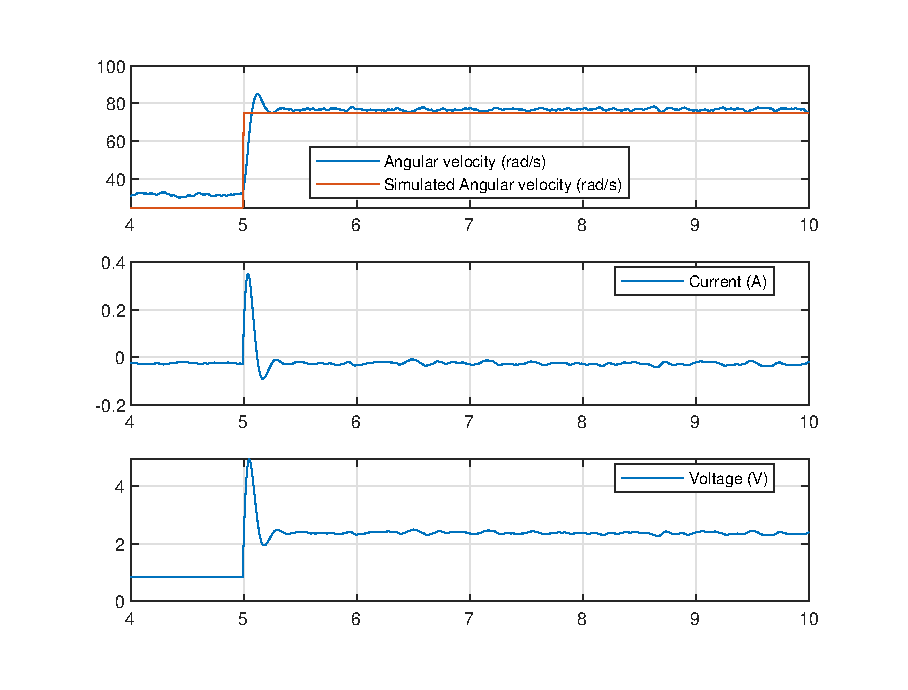
\includegraphics[width=\maxwidth{56.196688409433015em}]{figure_3.eps}
\end{center}


\matlabheading{\textit{Question 7 (0.5 marks)}}

\begin{par}
\begin{flushleft}
Based on the plot above, determine if all the requirements are satisfied. Justify your answer.
\end{flushleft}
\end{par}

\begin{matlabcode}
% The objective was to track a signal ωrefwhile satisfying the following requirements:
% • Overshoot less than 20%.
% • 5%-settling time less than 0.25 seconds.
% • Steady state gain of 1±5%.

% The 5% settling time is about 0.175 seconds based on the plots which is smaller \
% than 0.25 seconds so the settling time requirements are met.
% The OS% can be found as 11.33% which is less than 20% so OS requirements
% are met too. 

finalW = mean(w(t>=6));
finalWred = mean(wRef(t>=6));
SSgain = finalW/finalWred
\end{matlabcode}
\begin{matlaboutput}
SSgain = 1.0244
\end{matlaboutput}
\begin{matlabcode}

% We also find an ss gain of about 1.025 which lies in our error
% bound. So ss gain requirements are met too.
% All requirements are satisfied.

\end{matlabcode}


\matlabheading{\textit{Question 8 (1 mark)}}

\begin{par}
\begin{flushleft}
Can you tune the value of the gain $N_d$ and $K_d$ to get the required performance. 
\end{flushleft}
\end{par}

\begin{par}
\begin{flushleft}
When you finish tuning, plot the final graph and fill up your final performances.
\end{flushleft}
\end{par}

\begin{matlabcode}
NdTuned = Nd * 0.97;
KdTuned = [0.97 * Kd(1), 1.01* Kd(2)];

Motor.reset();
%  Run the experiment use
for n = 1:length(t)
    Motor.wait(t(n));
    w_ = Motor.velocity_final; % the final reading of velocity by sensor
    i_ = Motor.current_final; % the final reading of current by sensor
    
    if t(n) < TStart % We only run 
        v_ = wRef(n) / dcGainOL;
    else
        % Write the state feedback controller equation
        x = [w_; i_];
        v_ = NdTuned * wRef (n) - KdTuned * x;

    end
    Motor.input(v_);
end
Motor.off();

Motor.save(Students, 'Lab05.Q8');

% Get results of Virtual DC Motor
v = Motor.voltage(Motor.time <= T);
i = Motor.current(Motor.time <= T);
w = Motor.velocity(Motor.time <= T);
\end{matlabcode}


\begin{matlabcode}
% Plot new results
figure;
clf;

subplot(3, 1, 1)
title(sprintf('Student ID %s - Closed-loop tracking experiment (Tweaking); N = %04.2f; K=[%04.2f,%04.2f]', ...
    Students.ID, NdTuned, KdTuned));
% Superpose the angular velocity and the velocity reference
plot (t, w)
hold on
plot (t, wRef)
hold off

legend('Angular velocity (rad/s)', ...
    'Simulated Angular velocity (rad/s)', ...
    'Reference angular velocity (rad/s)', ...
    'location', 'best');
xlim([TStart - 1, T])
grid on

subplot(3, 1, 2)
% Plot current
plot (t, i)

legend('Current (A)', 'location', 'best');
xlim([TStart - 1, T])
grid on

subplot(3, 1, 3)
% Plot voltage
plot(t, v)

legend('Voltage (V)', 'location', 'best');
xlim([TStart - 1, T])
grid on
\end{matlabcode}
\begin{center}
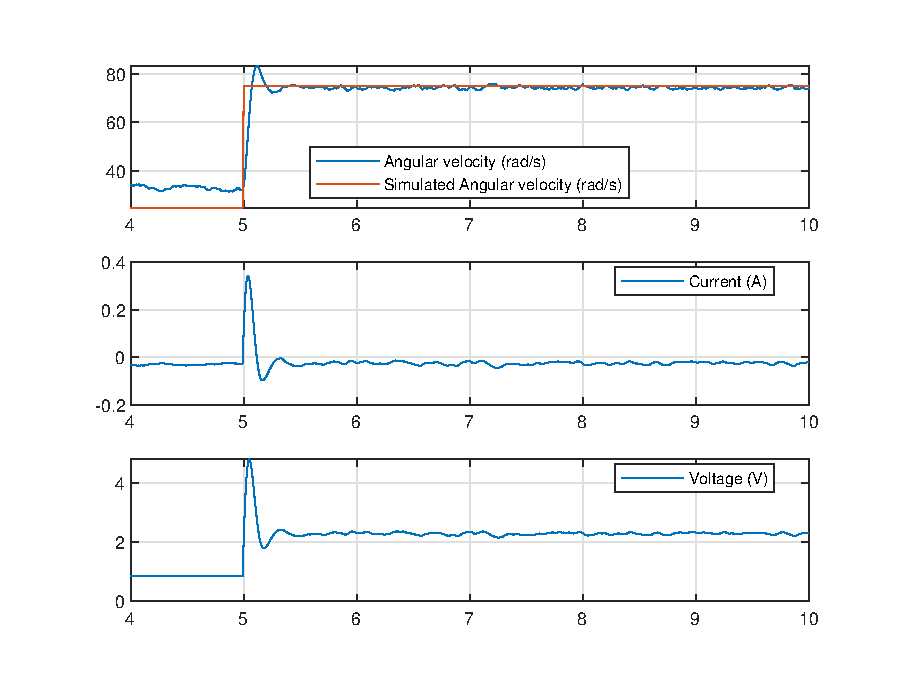
\includegraphics[width=\maxwidth{56.196688409433015em}]{figure_4.eps}
\end{center}


\begin{matlabcode}
% Final performance obtained:
stepinfo(w,t,"SettlingTimeThreshold", 0.05)
\end{matlabcode}
\begin{matlaboutput}
ans = 
        RiseTime: 5.0159
    SettlingTime: 5.1704
     SettlingMin: 69.0787
     SettlingMax: 83.3656
       Overshoot: 12.4267
      Undershoot: 0
            Peak: 83.3656
        PeakTime: 5.1200

\end{matlaboutput}
\begin{matlabcode}

finalW = mean(w(t>=6));
finalWred = mean(wRef(t>=6));
SSgain = finalW/finalWred
\end{matlabcode}
\begin{matlaboutput}
SSgain = 0.9902
\end{matlaboutput}
\begin{matlabcode}
steadyStateError = abs(SSgain - 1) * 100
\end{matlabcode}
\begin{matlaboutput}
steadyStateError = 0.9792
\end{matlaboutput}
\begin{matlabcode}
settlingTime = 0.17
\end{matlabcode}
\begin{matlaboutput}
settlingTime = 0.1700
\end{matlaboutput}
\begin{matlabcode}
overshoot = 12.52
\end{matlabcode}
\begin{matlaboutput}
overshoot = 12.5200
\end{matlaboutput}
\begin{matlabcode}

if settlingTime <= 0.25 && ...
        overshoot <= 20 && ...
        steadyStateError <= 1
    disp('All requirements are satisfied')
else
    disp('Not all requirements are satisfied')
end
\end{matlabcode}
\begin{matlaboutput}
All requirements are satisfied
\end{matlaboutput}

\end{document}
